\documentclass[10pt]{beamer}

% Packages
\usepackage[utf8]{inputenc}
\usepackage[T1]{fontenc}
\usepackage{amsmath, amssymb, amsthm}
\usepackage{graphicx}
\usepackage{booktabs}
\usepackage{hyperref}
\usepackage{tikz}
\usetikzlibrary{shapes,arrows,positioning}

% Theme settings
\usetheme{default}
\usecolortheme{default}
\usefonttheme{professionalfonts}

\definecolor{ImperialBlue}{RGB}{0, 62, 116}
\definecolor{DarkGray}{RGB}{51, 51, 51}
\definecolor{LightGray}{RGB}{245, 245, 245}
\definecolor{AccentOrange}{RGB}{214, 96, 77}
\definecolor{AccentGreen}{RGB}{46, 139, 87}

% Apply colors
\setbeamercolor{frametitle}{fg=ImperialBlue, bg=white}
\setbeamercolor{title}{fg=ImperialBlue}
\setbeamercolor{structure}{fg=ImperialBlue}
\setbeamercolor{normal text}{fg=DarkGray}
\setbeamercolor{block title}{fg=white, bg=ImperialBlue}
\setbeamercolor{block body}{fg=DarkGray, bg=LightGray}
\setbeamercolor{itemize item}{fg=ImperialBlue}
\setbeamercolor{enumerate item}{fg=ImperialBlue}

% Remove navigation symbols
\setbeamertemplate{navigation symbols}{}

% Customize frame title
\setbeamertemplate{frametitle}{
  \vspace{0.5em}
  \insertframetitle
  \vspace{0.3em}
}

% Customize itemize
\setbeamertemplate{itemize items}[circle]
\setlength{\leftmargini}{1.5em}

% Footer
\setbeamertemplate{footline}{
  \leavevmode%
  \hbox{%
  \begin{beamercolorbox}[wd=.333333\paperwidth,ht=2.25ex,dp=1ex,left]{author in head/foot}%
    \hspace{1em}\usebeamerfont{author in head/foot}\insertshortauthor
  \end{beamercolorbox}%
  \begin{beamercolorbox}[wd=.333333\paperwidth,ht=2.25ex,dp=1ex,center]{title in head/foot}%
    \usebeamerfont{title in head/foot}\insertshorttitle
  \end{beamercolorbox}%
  \begin{beamercolorbox}[wd=.333333\paperwidth,ht=2.25ex,dp=1ex,right]{date in head/foot}%
    \usebeamerfont{date in head/foot}\insertshortdate{}\hspace*{2em}
    \insertframenumber{} / \inserttotalframenumber\hspace*{2ex} 
  \end{beamercolorbox}}%
  \vskip0pt%
}

% Title page customization
\setbeamertemplate{title page}{
  \vbox{}
  \vfill
  \begingroup
    \centering
    {\usebeamercolor[fg]{title}\usebeamerfont{title}\inserttitle\par}
    \vskip0.5em
    {\usebeamercolor[fg]{subtitle}\usebeamerfont{subtitle}\insertsubtitle\par}
    \vskip2em
    {\usebeamercolor[fg]{author}\usebeamerfont{author}\insertauthor\par}
    \vskip0.5em
    {\usebeamercolor[fg]{institute}\usebeamerfont{institute}\insertinstitute\par}
    \vskip1em
    {\usebeamercolor[fg]{date}\usebeamerfont{date}\insertdate\par}
  \endgroup
  \vfill
}

% Commands for highlighting
\newcommand{\emphbox}[1]{\colorbox{LightGray}{\textcolor{DarkGray}{#1}}}
\newcommand{\highlight}[1]{\textcolor{AccentOrange}{\textbf{#1}}}
\newcommand{\good}[1]{\textcolor{AccentGreen}{#1}}
\newcommand{\bad}[1]{\textcolor{AccentOrange}{#1}}

%----------------------------------------------------------------------------------------
\title{Decentralised Finance (DeFi)}
\subtitle{ECOM215: Blockchain Economics and Digital Assets}

\author{Dr Daniele Bianchi}
\institute{Queen Mary, University of London}
\date{Semester B, 2025/2026}
%----------------------------------------------------------------------------------------

\begin{document}

\AtBeginSection[]{
  \begin{frame}[plain]
    \vfill
    \begin{center}
      {\Large\color{ImperialBlue}\insertsection}
    \end{center}
    \vfill
  \end{frame}
}

\begin{frame}[plain]
  \titlepage
\end{frame}

\begin{frame}{Today's Agenda}
  \tableofcontents
\end{frame}

%----------------------------------------------------------------------------------------
\section{What is DeFi?}
%----------------------------------------------------------------------------------------

\begin{frame}{The DeFi Vision}
  \begin{block}{Decentralised Finance (DeFi)}
    Financial services---lending, borrowing, trading, insurance---built on smart contracts instead of traditional intermediaries.
  \end{block}
  
  \vspace{1em}
  \textbf{Traditional finance}: Banks, brokers, and exchanges sit between you and financial services. They custody assets, match orders, assess credit, and take fees.
  
  \vspace{1em}
  \textbf{DeFi}: Smart contracts perform these functions. Code replaces institutions (see Week 3).
  
  \vspace{1em}
  \textbf{Key properties}:
  \begin{itemize}
    \item \textbf{Permissionless}: Anyone with a wallet can ``plug-in''
    \item \textbf{Non-custodial}: Users retain control of their assets
    \item \textbf{Transparent}: All transactions are publicly visible (e.g., etherscan.io)
    \item \textbf{Composable}: Protocols can be combined like building blocks
  \end{itemize}
\end{frame}

\begin{frame}{DeFi by the Numbers}
  \textbf{Total Value Locked (TVL)}: how much capital is deposited in DeFi protocols---the standard metric for DeFi adoption.
  \begin{figure}
    \centering
    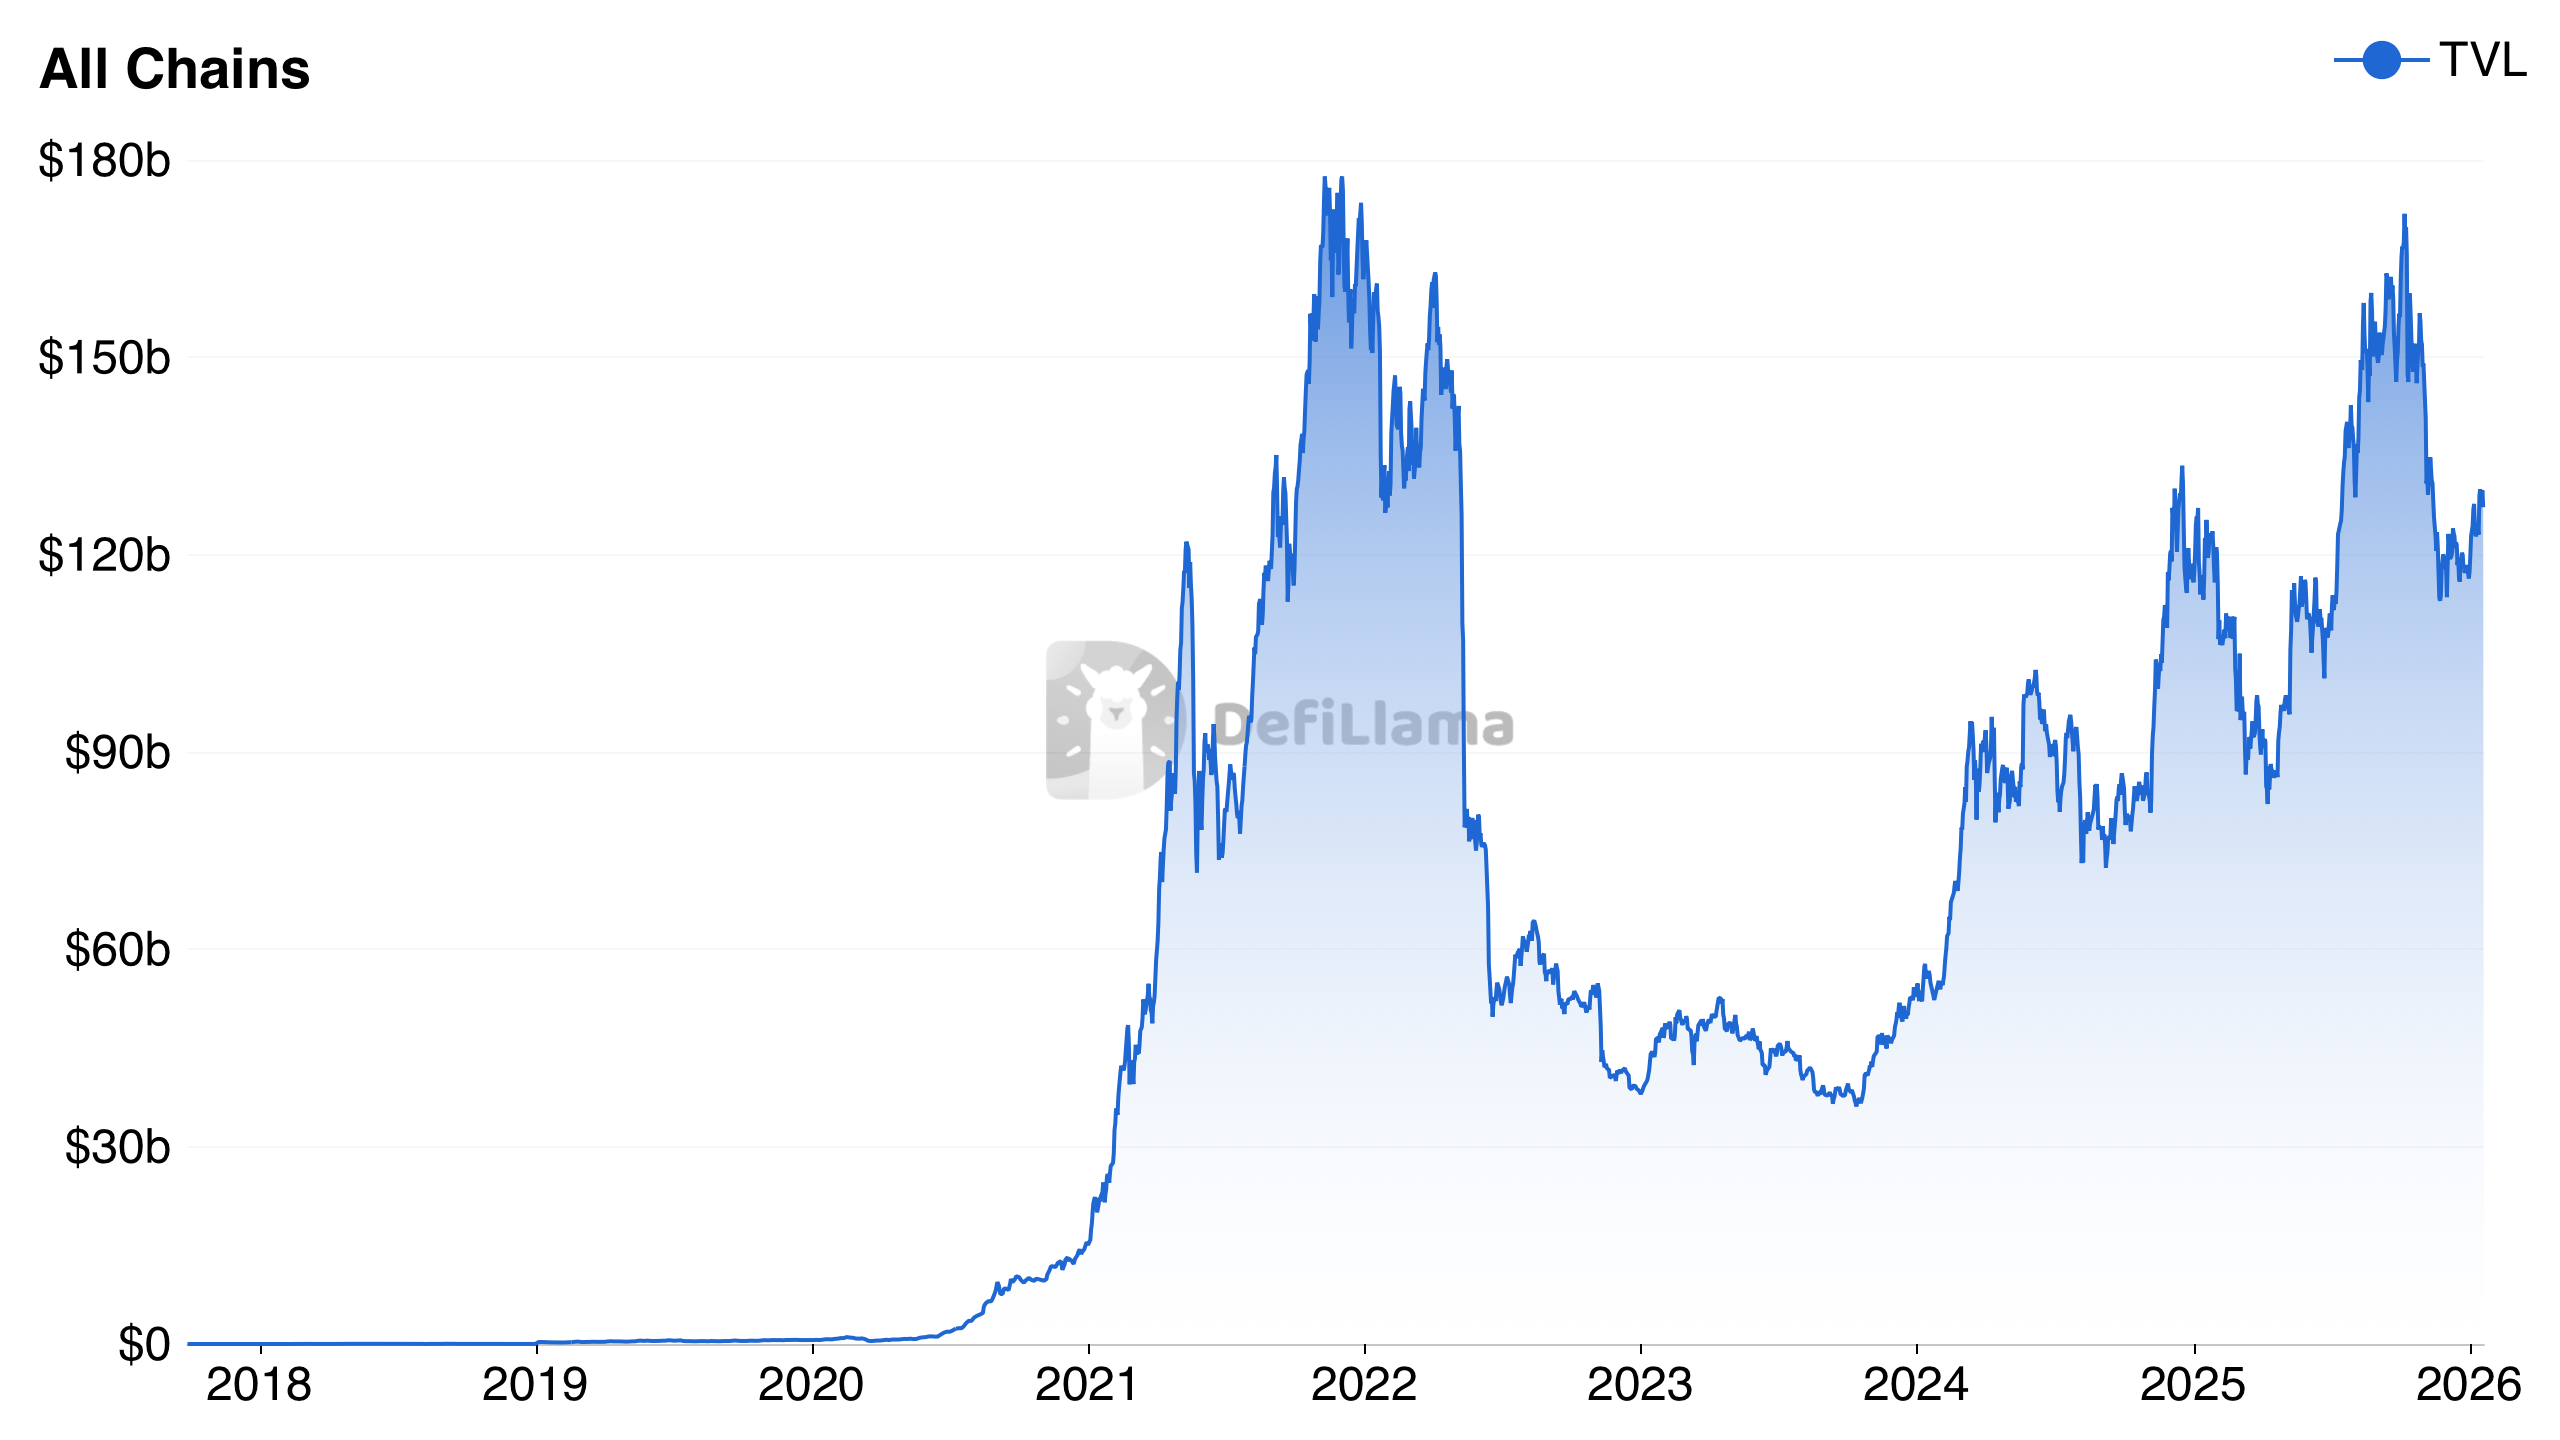
\includegraphics[width=.85\textwidth]{Figures/TVL DeFi.png}
  \end{figure}
  \textbf{Perspective}: Global banking assets exceed \$180 \textit{trillion}. DeFi remains tiny, but is growing.
\end{frame}

\begin{frame}{DeFi by the Numbers}
  \begin{figure}
    \centering
    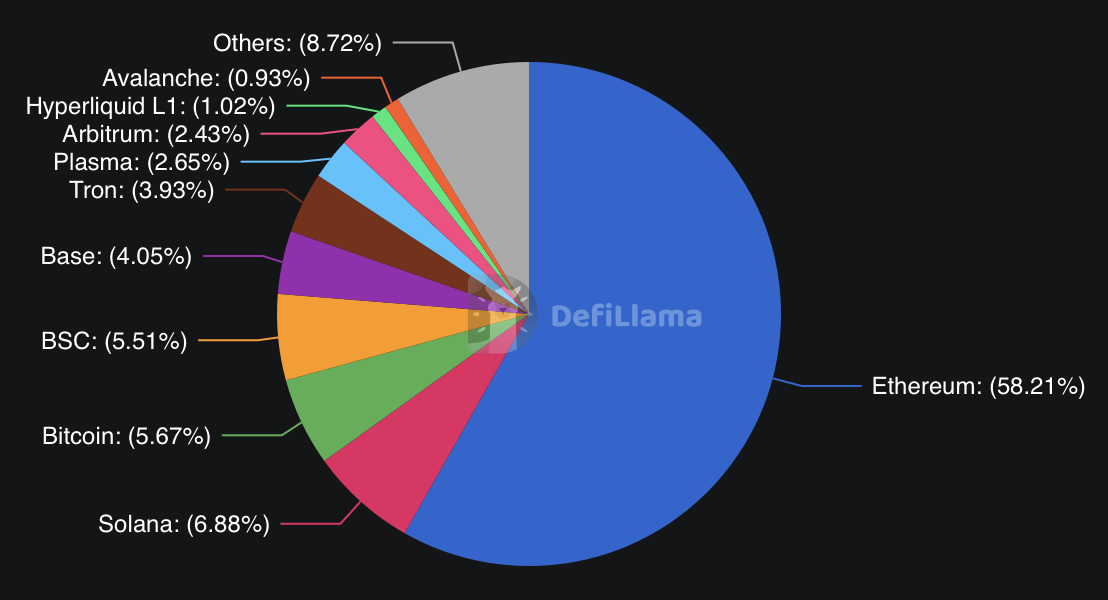
\includegraphics[width=.9\textwidth]{Figures/TVL DeFi ByChain.png}
  \end{figure}
  \textbf{Perspective}: Ethereum holds $\approx$60\% of total DeFi TVL. Other chains (Solana, BNB Chain) account for $\approx$20\% combined, while Layer 2s (Arbitrum, Optimism) hold a growing share.
\end{frame}


\begin{frame}{``Money Legos'': Composability}
  DeFi protocols can interact with each other, creating complex financial products from simple building blocks.
  
  \vspace{1em}
  \textbf{Example}: A single transaction might:
  \begin{enumerate}
    \item Swap ETH for USDC on Uniswap
    \item Deposit USDC into Aave as collateral
    \item Borrow DAI against that collateral
    \item Deposit DAI into a yield aggregator
  \end{enumerate}
  
  \vspace{0.5em}
  All of this happens atomically---either everything succeeds or nothing does.
  
  \vspace{1em}
  \textbf{Benefits}: Innovation, capital efficiency, user choice
  
  \textbf{Risks}: Failures cascade. A bug in one protocol can affect all protocols that depend on it.
  
  \vspace{0.5em}
  This interconnectedness is both DeFi's greatest strength and its greatest vulnerability.
\end{frame}

\begin{frame}{DeFi vs Traditional Finance: Key Differences}
  \begin{center}
  \begin{tabular}{lcc}
    \toprule
    & \textbf{Traditional Finance} & \textbf{DeFi} \\
    \midrule
    Access & Permissioned (KYC) & Permissionless \\
    Custody & Institutions hold assets & Users hold assets \\
    Operating hours & Business hours & 24/7/365 \\
    Settlement & T+2 days (typical) & Minutes \\
    Transparency & Opaque & Fully public \\
    Recourse & Legal system & Code is law \\
    \midrule
    Regulation & Extensive & Minimal/unclear \\
    Insurance & FDIC, etc. & Limited/none \\
    Reversibility & Possible & Generally not \\
    \bottomrule
  \end{tabular}
  \end{center}
  
  \vspace{0.5em}
  Neither is strictly better---they involve different trade-offs. DeFi offers access and transparency; traditional finance offers protections and recourse.
\end{frame}

%----------------------------------------------------------------------------------------
\section{Automated Market Makers (AMMs)}
%----------------------------------------------------------------------------------------

\begin{frame}{The Problem AMMs Solve}
  \textbf{Traditional exchanges} use order books:
  \begin{itemize}
    \item Buyers post bids, sellers post asks
    \item Market makers provide liquidity by quoting both sides
    \item Orders match when prices meet
  \end{itemize}
  
  \vspace{0.5em}
  \textbf{Problem for DeFi}: Order books are expensive on-chain. Every order placement, cancellation, and modification costs gas fees. Professional market makers need speed that blockchains cannot provide.
  
  \vspace{1em}
  \textbf{The AMM solution}: Replace the order book with a mathematical formula that automatically determines prices based on supply and demand.
  
  \vspace{0.5em}
  \begin{block}{Automated Market Maker}
    A smart contract that holds reserves of two (or more) tokens and allows anyone to trade against those reserves at a price determined by an algorithm.
  \end{block}
\end{frame}

\begin{frame}{How Uniswap Works: The Constant Product Formula}
  Uniswap (launched 2018) pioneered the \highlight{constant product} AMM:
  
  \vspace{0.5em}
  \begin{center}
    \Large $x \cdot y = k$
  \end{center}
  
  Where:
  \begin{itemize}
    \item $x$ = quantity of Token A in the pool
    \item $y$ = quantity of Token B in the pool
    \item $k$ = constant (the ``invariant'')
  \end{itemize}
  
  \vspace{1em}
  \textbf{The rule}: After any trade, the product $x \cdot y$ must remain equal to $k$.
  
  \vspace{1em}
  \textbf{Example}: A pool has 100 ETH and 200,000 USDC.
  \begin{itemize}
    \item $k = 100 \times 200{,}000 = 20{,}000{,}000$
    \item Implied price: 200,000 / 100 = 2,000 USDC per ETH
  \end{itemize}
\end{frame}

\begin{frame}{Trading Against the Pool}
  \textbf{Example}: You want to buy 1 ETH from the pool.
  
  \vspace{0.5em}
  \textbf{Starting state}: 100 ETH, 200,000 USDC
  \begin{itemize}
    \item Constant product: $k = 100 \times 200{,}000 = 20{,}000{,}000$
    \item Current price: $\frac{200{,}000}{100} = 2{,}000$ USDC per ETH
  \end{itemize}
  
  \vspace{0.5em}
  \textbf{After you remove 1 ETH}: Pool has 99 ETH. How much USDC must remain?
  \[
  99 \times y = 20{,}000{,}000 \implies y = \frac{20{,}000{,}000}{99} = 202{,}020.20 \text{ USDC}
  \]
  
  \vspace{0.5em}
  \textbf{Your cost}: The pool had 200,000 USDC, now needs 202,020.20 USDC.
  \[
  \text{You pay: } 202{,}020.20 - 200{,}000 = \highlight{2{,}020.20 \text{ USDC}}
  \]
  
  \vspace{0.5em}
  \textbf{Effective price}: $\frac{2{,}020.20}{1} = 2{,}020.20$ USDC per ETH
  
  \vspace{0.5em}
  You paid 20.20 USDC \textit{more} than the initial price of 2,000. This premium is \highlight{slippage}---the cost of moving the pool's reserves.
\end{frame}

\begin{frame}{Why Does Slippage Occur?}
  \textbf{The constant product rule} means larger trades get worse prices.
  
  \vspace{0.5em}
  \textbf{Example}: What if you want to buy 10 ETH instead of 1?
  
  \vspace{0.5em}
  Pool after trade: $100 - 10 = 90$ ETH remain.
  \[
  90 \times y = 20{,}000{,}000 \implies y = \frac{20{,}000{,}000}{90} = 222{,}222.22 \text{ USDC}
  \]
  
  \vspace{0.5em}
  \textbf{Your cost}: $222{,}222.22 - 200{,}000 = 22{,}222.22$ USDC for 10 ETH.
  
  \vspace{0.5em}
  \textbf{Effective price}: $\frac{22{,}222.22}{10} = 2{,}222.22$ USDC per ETH
  
  \vspace{1em}
  \begin{center}
  \begin{tabular}{ccc}
    \toprule
    \textbf{Trade Size} & \textbf{Effective Price} & \textbf{Slippage} \\
    \midrule
    1 ETH & 2,020.20 & +1.01\% \\
    10 ETH & 2,222.22 & +11.1\% \\
    \bottomrule
  \end{tabular}
  \end{center}
  
  \vspace{0.5em}
  This is how the AMM automatically adjusts prices to reflect demand.
\end{frame}

\begin{frame}{Visualising the Constant Product Curve}
  \begin{center}
  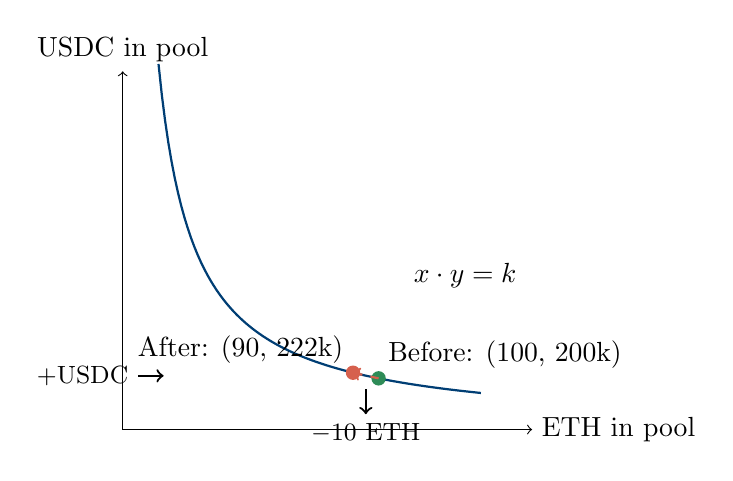
\begin{tikzpicture}[scale=0.65]
    % Axes
    \draw[->] (0,0) -- (8,0) node[right] {ETH in pool};
    \draw[->] (0,0) -- (0,7) node[above] {USDC in pool};
    
    % Curve (x*y = k, scaled: using x*y = 20 for visibility)
    \draw[thick, ImperialBlue, domain=0.7:7, samples=100] plot (\x, {5/\x});
    
    % Points matching our example (scaled: 100 ETH -> 5, 99 ETH -> 4.95)
    % At x=5: y=1 (representing 100 ETH, 200k USDC)
    % At x=4.95: y=1.0101 (representing 99 ETH, 202k USDC)
    \fill[AccentGreen] (5,1) circle (4pt);
    \node[above right] at (5,1) {Before: (100, 200k)};
    
    \fill[AccentOrange] (4.5,1.11) circle (4pt);
    \node[above left] at (4.5,1.11) {After: (90, 222k)};
    
    % Arrow showing trade direction
    \draw[->, thick, dashed, AccentOrange] (5,1) -- (4.5,1.11);
    
    % Annotation
    \node[right] at (5.5,3) {$x \cdot y = k$};
    
    % Trade annotation
    \draw[<-, thick] (4.75, 0.3) -- (4.75, 0.8);
    \node[below] at (4.75, 0.3) {\small $-$10 ETH};
    \draw[->, thick] (0.3, 1.05) -- (0.8, 1.05);
    \node[left] at (0.3, 1.05) {\small $+$USDC};
  \end{tikzpicture}
  \end{center}
  
  \vspace{0.3em}
  When you buy ETH (move left on x-axis), you add USDC (move up on y-axis) to stay on the curve.
  
  \vspace{0.3em}
  \textbf{Key property}: The curve never touches the axes---you can never fully drain one token. As reserves approach zero, price approaches infinity.
\end{frame}

\begin{frame}{Liquidity Providers (LPs)}
  \textbf{Where do pool reserves come from?} Anyone can deposit tokens and become a \highlight{liquidity provider} (LP).
  
  \vspace{0.5em}
  \textbf{Example}: A pool has 100 ETH + 200,000 USDC (worth \$400,000 at current prices). You want to add liquidity.
  
  \vspace{0.5em}
  \textbf{Rule}: You must deposit both tokens in the current pool ratio.
  \begin{itemize}
    \item Current ratio: $\frac{200{,}000}{100} = 2{,}000$ USDC per ETH
    \item To deposit 1 ETH, you must also deposit 2,000 USDC
  \end{itemize}
  
  \vspace{0.5em}
  \textbf{Your ownership share}:
  \[
  \text{Share} = \frac{\text{Your deposit}}{\text{Total pool after deposit}} = \frac{1 \text{ ETH}}{101 \text{ ETH}} \approx 0.99\%
  \]
  
  \vspace{0.5em}
  \textbf{You receive}: LP tokens representing your 0.99\% claim on the pool.
  
  \vspace{0.5em}
  \textbf{How LPs earn}: Traders pay a fee (typically 0.3\%) on each swap. Fees stay in the pool, increasing its value. Your LP tokens entitle you to your share of the growing pool.
\end{frame}

\begin{frame}{LP Returns: An Example}
  \textbf{Setup}: You own 1\% of a pool. Pool starts with 100 ETH + 200,000 USDC.
  
  \vspace{0.5em}
  \textbf{Your position value} (at ETH = \$2,000):
  \[
  1\% \times (100 \times \$2{,}000 + \$200{,}000) = 1\% \times \$400{,}000 = \$4{,}000
  \]
  
  \vspace{0.5em}
  \textbf{Trading activity}: Over one month, \$10 million in volume passes through the pool at a 0.3\% fee.
  \[
  \text{Total fees collected} = \$10{,}000{,}000 \times 0.003 = \$30{,}000
  \]
  
  \vspace{0.5em}
  \textbf{Your share of fees}: $\$30{,}000 \times 1\% = \$300$
  
  \vspace{0.5em}
  \textbf{Annualised return} (if this rate continues):
  \[
  \text{APR} = \frac{\$300 \times 12}{\$4{,}000} = 90\%
  \]
  
  \vspace{0.5em}
  \textbf{Sounds great---but there's a catch}: While you earned fees, the pool composition changed as traders swapped. If prices moved, your position may have \highlight{underperformed} simply holding. This is \highlight{impermanent loss}.
\end{frame}

\begin{frame}{Impermanent Loss: Setup}
  \textbf{Scenario}: You provide liquidity when ETH = 2,000 USDC.
  
  \vspace{0.5em}
  \textbf{Your initial deposit}:
  \begin{itemize}
    \item 1 ETH + 2,000 USDC = \$4,000 total value
    \item You own some share of the pool (exact \% doesn't matter for this calculation)
  \end{itemize}
  
  \vspace{0.5em}
  \textbf{Later}: ETH price rises to 4,000 USDC (doubles).
  
  \vspace{0.5em}
  \textbf{Question}: What is your LP position worth now?
  
  \vspace{0.5em}
  \textbf{Key insight}: Arbitrageurs will trade against the pool until the pool price matches the external market price. This \textit{rebalances} the pool composition.
  
  \vspace{0.5em}
  The pool must satisfy two conditions simultaneously:
  \begin{enumerate}
    \item Constant product: $x \cdot y = k$ (unchanged)
    \item Market price: $\frac{y}{x} = 4{,}000$ (new external price)
  \end{enumerate}
\end{frame}

\begin{frame}{Impermanent Loss: The Rebalancing Calculation}
  \textbf{Finding the new pool composition}:
  
  \vspace{0.5em}
  Let the pool have $x$ ETH and $y$ USDC after rebalancing.
  
  \begin{align*}
    x \cdot y &= k = 1 \times 2{,}000 = 2{,}000 && \text{(constant product)} \\[0.5em]
    \frac{y}{x} &= 4{,}000 && \text{(new market price)}
  \end{align*}
  
  \vspace{0.3em}
  From the second equation: $y = 4{,}000 \cdot x$
  
  \vspace{0.3em}
  Substitute into the first equation:
  \[
  x \cdot (4{,}000 \cdot x) = 2{,}000 \implies x^2 = \frac{2{,}000}{4{,}000} = 0.5 \implies x = \sqrt{0.5} \approx \highlight{0.707 \text{ ETH}}
  \]
  
  \vspace{0.3em}
  And therefore:
  \[
  y = 4{,}000 \times 0.707 = \highlight{2{,}828 \text{ USDC}}
  \]
  
  \vspace{0.5em}
  \textbf{What happened?} Arbitrageurs bought ETH from the pool (cheap relative to market), removing ETH and adding USDC until prices equalised.
\end{frame}

\begin{frame}{Impermanent Loss: The Cost}
  \textbf{Your LP position after rebalancing}:
  \begin{itemize}
    \item 0.707 ETH @ \$4,000 = \$2,828
    \item 2,828 USDC = \$2,828
    \item \textbf{Total}: \$5,656
  \end{itemize}
  
  \vspace{0.5em}
  \textbf{If you had just held the original tokens}:
  \begin{itemize}
    \item 1 ETH @ \$4,000 = \$4,000
    \item 2,000 USDC = \$2,000
    \item \textbf{Total}: \$6,000
  \end{itemize}
  
  \vspace{0.5em}
  \textbf{Impermanent loss}:
  \[
  \$6{,}000 - \$5{,}656 = \highlight{\$344} \quad \text{(5.7\% of hold value)}
  \]
  
  \vspace{0.5em}
  \textbf{Why ``impermanent''?} If ETH returns to \$2,000, the pool rebalances back to 1 ETH + 2,000 USDC, and the loss disappears.
  
  \vspace{0.5em}
  \textbf{But}: If you withdraw while prices have diverged, the loss becomes \textit{permanent}. LPs must earn enough fees to compensate for this risk.
\end{frame}

\begin{frame}{Impermanent Loss: The General Pattern}
  \begin{center}
  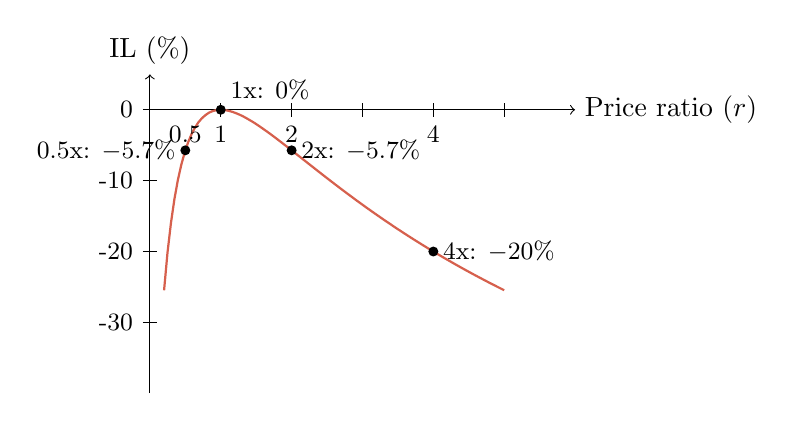
\begin{tikzpicture}[scale=0.9]
    % Axes
    \draw[->] (0,0) -- (6,0) node[right] {Price ratio ($r$)};
    \draw[->] (0,-4) -- (0,0.5) node[above] {IL (\%)};
    
    % Y-axis labels
    \foreach \y/\label in {0/0, -1/-10, -2/-20, -3/-30} {
      \draw (-0.1,\y) -- (0.1,\y);
      \node[left] at (-0.1,\y) {\small \label};
    }
    
    % X-axis tick marks
    \foreach \x in {1,2,3,4,5} {
      \draw (\x,-0.1) -- (\x,0.1);
    }
    
    % IL curve: IL = 2*sqrt(r)/(1+r) - 1
    % Scale: x-axis is price ratio r, y-axis is IL*10 (so -20% = -2)
    \draw[thick, AccentOrange, domain=0.2:5, samples=100] 
      plot (\x, {10*(2*sqrt(\x)/(1+\x) - 1)});
    
    % Reference points (y = IL * 10)
    \fill (1,0) circle (2pt) node[above right] {\small 1x: 0\%};
    \fill (2,-0.572) circle (2pt) node[right] {\small 2x: $-5.7\%$};
    \fill (4,-2.0) circle (2pt) node[right] {\small 4x: $-20\%$};
    \fill (0.5,-0.572) circle (2pt) node[left] {\small 0.5x: $-5.7\%$};
    
    % X-axis labels
    \node[below] at (0.5,-0.1) {\small 0.5};
    \node[below] at (1,-0.1) {\small 1};
    \node[below] at (2,-0.1) {\small 2};
    \node[below] at (4,-0.1) {\small 4};
  \end{tikzpicture}
  \end{center}
  
  \vspace{0.3em}
  \textbf{Key observations}:
  \begin{itemize}
    \item IL depends on price \textit{divergence}, not direction (2x up = 0.5x down)
    \item IL accelerates with larger price moves
    \item At 5x price change: IL $\approx$ 25\%. At 10x: IL $\approx$ 42\%.
  \end{itemize}
  
  \vspace{0.3em}
  \textbf{Implication}: LPs in volatile pairs (e.g., ETH/USDC) face higher IL than stable pairs (e.g., USDC/USDT). This explains APR differences across pools.
\end{frame}

\begin{frame}{Interpreting LP Yields: A Real Example}
  \begin{figure}
    \centering
    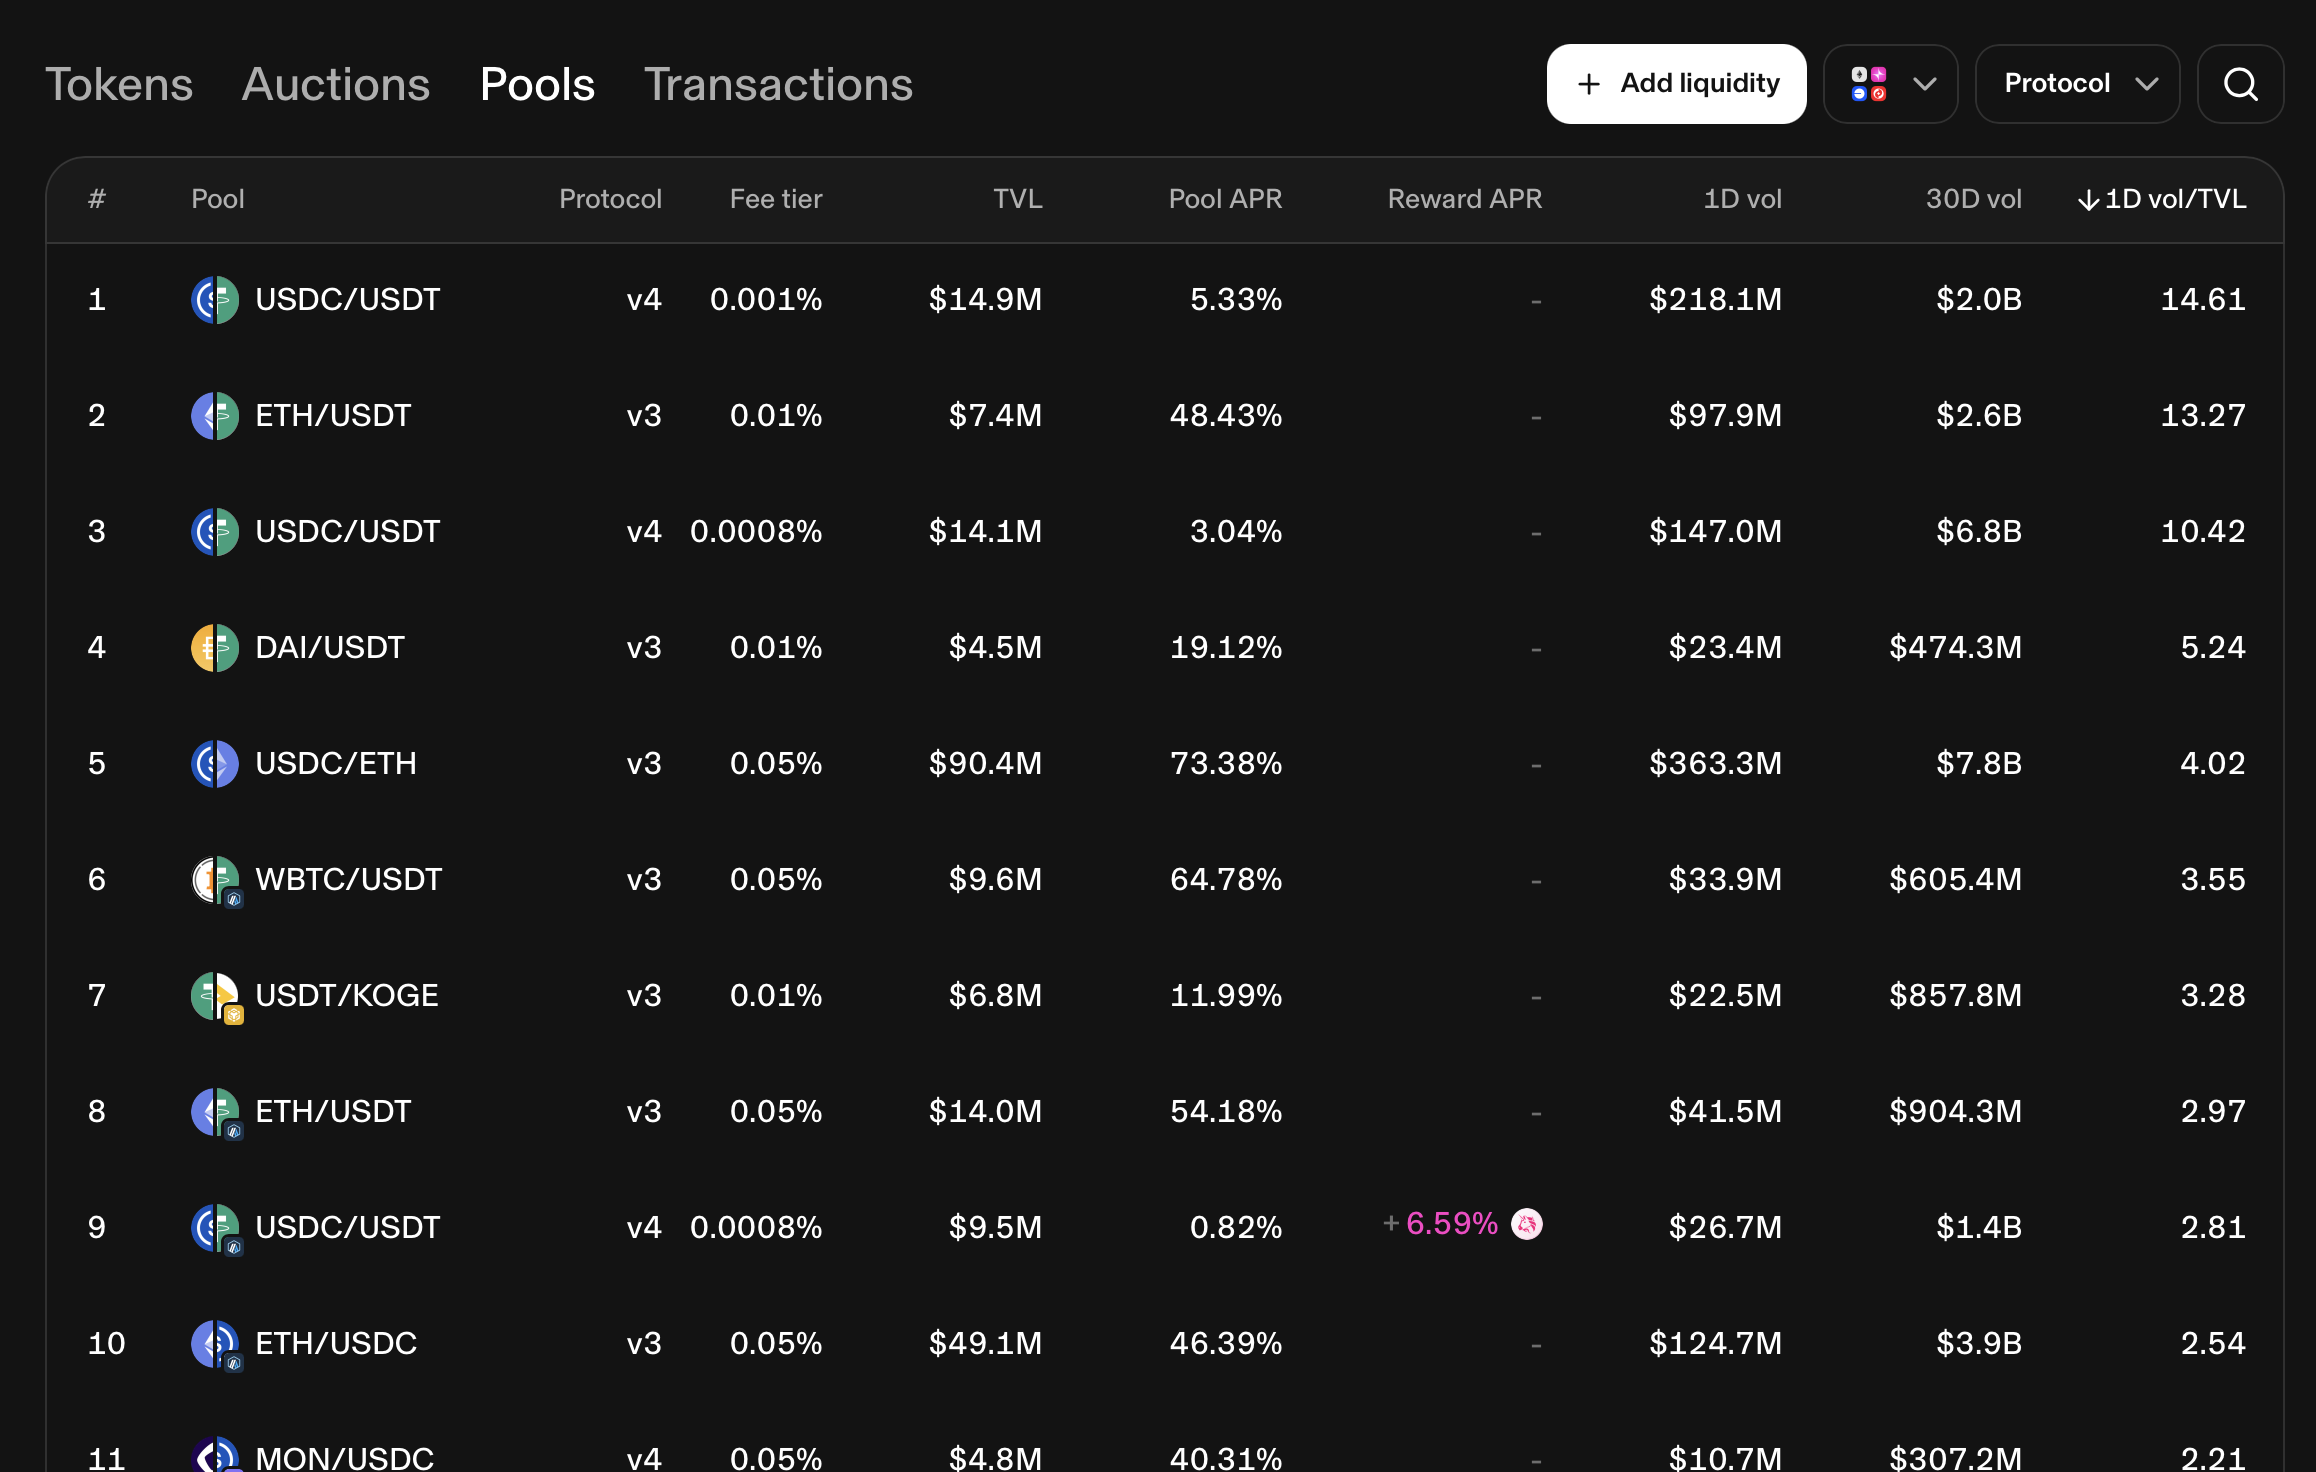
\includegraphics[width=.8\textwidth]{Figures/uniswap_pools.png}
  \end{figure}
  \textbf{Source}: Uniswap pool data, sorted by 1-day volume/TVL ratio (February 2026).
\end{frame}

\begin{frame}{Interpreting LP Yields: A Real Example}
  \textbf{Key columns}:
  \begin{itemize}
    \item \textbf{Fee tier}: What LPs earn per swap (0.0008\% to 0.05\%)
    \item \textbf{TVL}: Total capital deposited by LPs
    \item \textbf{Pool APR}: Annualised fee income relative to TVL
    \item \textbf{1D vol/TVL}: Daily trading volume as multiple of pool size
  \end{itemize}
  
  \vspace{0.5em}
  \textbf{The fee income formula}:
  \[
  \text{Pool APR} \approx \text{Fee Tier} \times \frac{\text{Volume}}{\text{TVL}} \times 365
  \]
  
  \vspace{0.5em}
  \textbf{Compare three pools}:
  \begin{center}
  \small
  \begin{tabular}{lcccl}
    \toprule
    \textbf{Pool} & \textbf{Fee} & \textbf{Vol/TVL} & \textbf{APR} & \textbf{Why?} \\
    \midrule
    USDC/USDT & 0.001\% & 14.61 & 5.3\% & High turnover, minimal IL risk \\
    ETH/USDT & 0.01\% & 13.27 & 48.4\% & Similar turnover, \highlight{IL risk} \\
    USDC/ETH & 0.05\% & 4.02 & 73.4\% & Lower turnover, higher fee + IL \\
    \bottomrule
  \end{tabular}
  \end{center}
  
  \vspace{0.3em}
  \textbf{Lesson}: High APR compensates for impermanent loss risk---not free money.
\end{frame}


\begin{frame}{AMM Landscape}
  \textbf{Uniswap} remains dominant, but variations exist:
  
  \vspace{1em}
  \begin{center}
  \begin{tabular}{lp{6cm}}
    \toprule
    \textbf{Protocol} & \textbf{Innovation} \\
    \midrule
    Uniswap v2 & Basic constant product \\
    Uniswap v3 & Concentrated liquidity (LPs choose price ranges) \\
    Curve & Optimised for stablecoin swaps (lower slippage) \\
    Balancer & Multi-token pools with custom weights \\
    \bottomrule
  \end{tabular}
  \end{center}
  
  \vspace{1em}
  
  \textbf{DEX vs CEX}: Decentralised exchanges handle $\approx$15--20\% of crypto spot trading volume. The majority still takes place on centralised exchanges (Binance, Coinbase).
\end{frame}

\begin{frame}{AMM Landscape}
  \begin{figure}
    \centering
    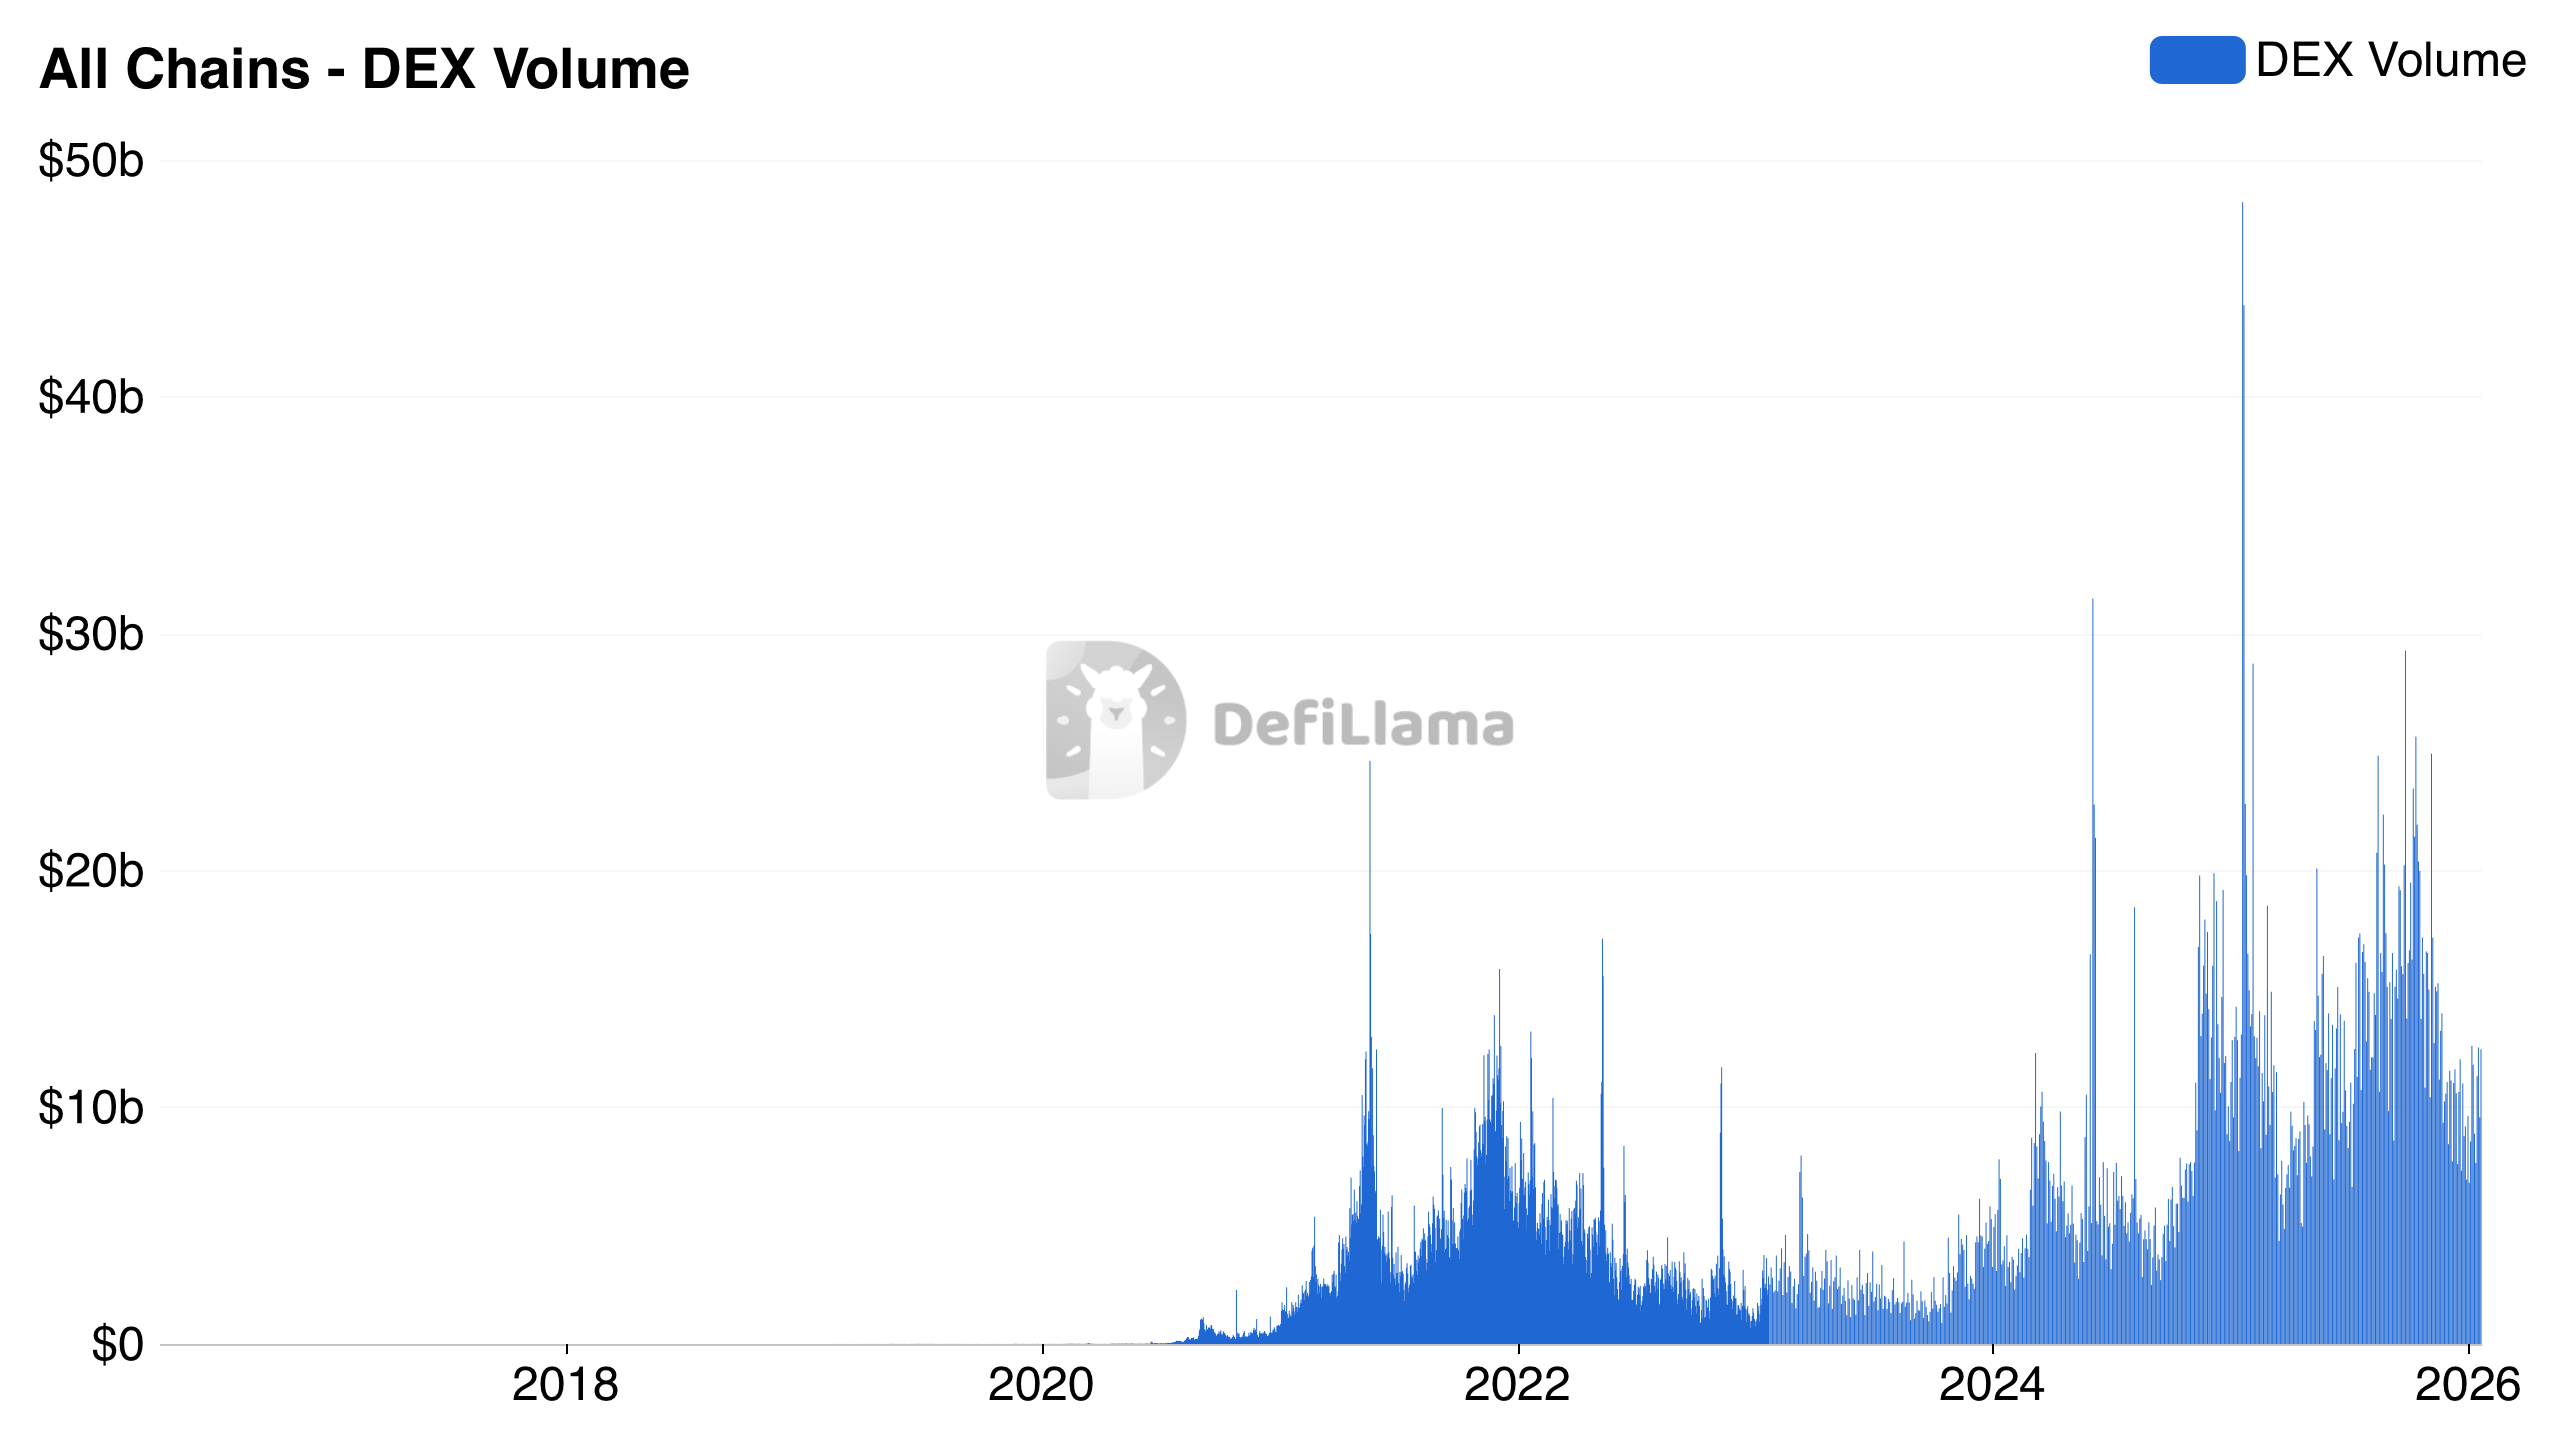
\includegraphics[width=1\textwidth]{Figures/DEX Volume.png}
  \end{figure}
  \textbf{Perspective}: Trading volume on DEXs is a tiny fraction of, for example, equity markets (which are measured in trillions of dollars).
\end{frame}


\begin{frame}{AMM Landscape}
  \begin{figure}
    \centering
    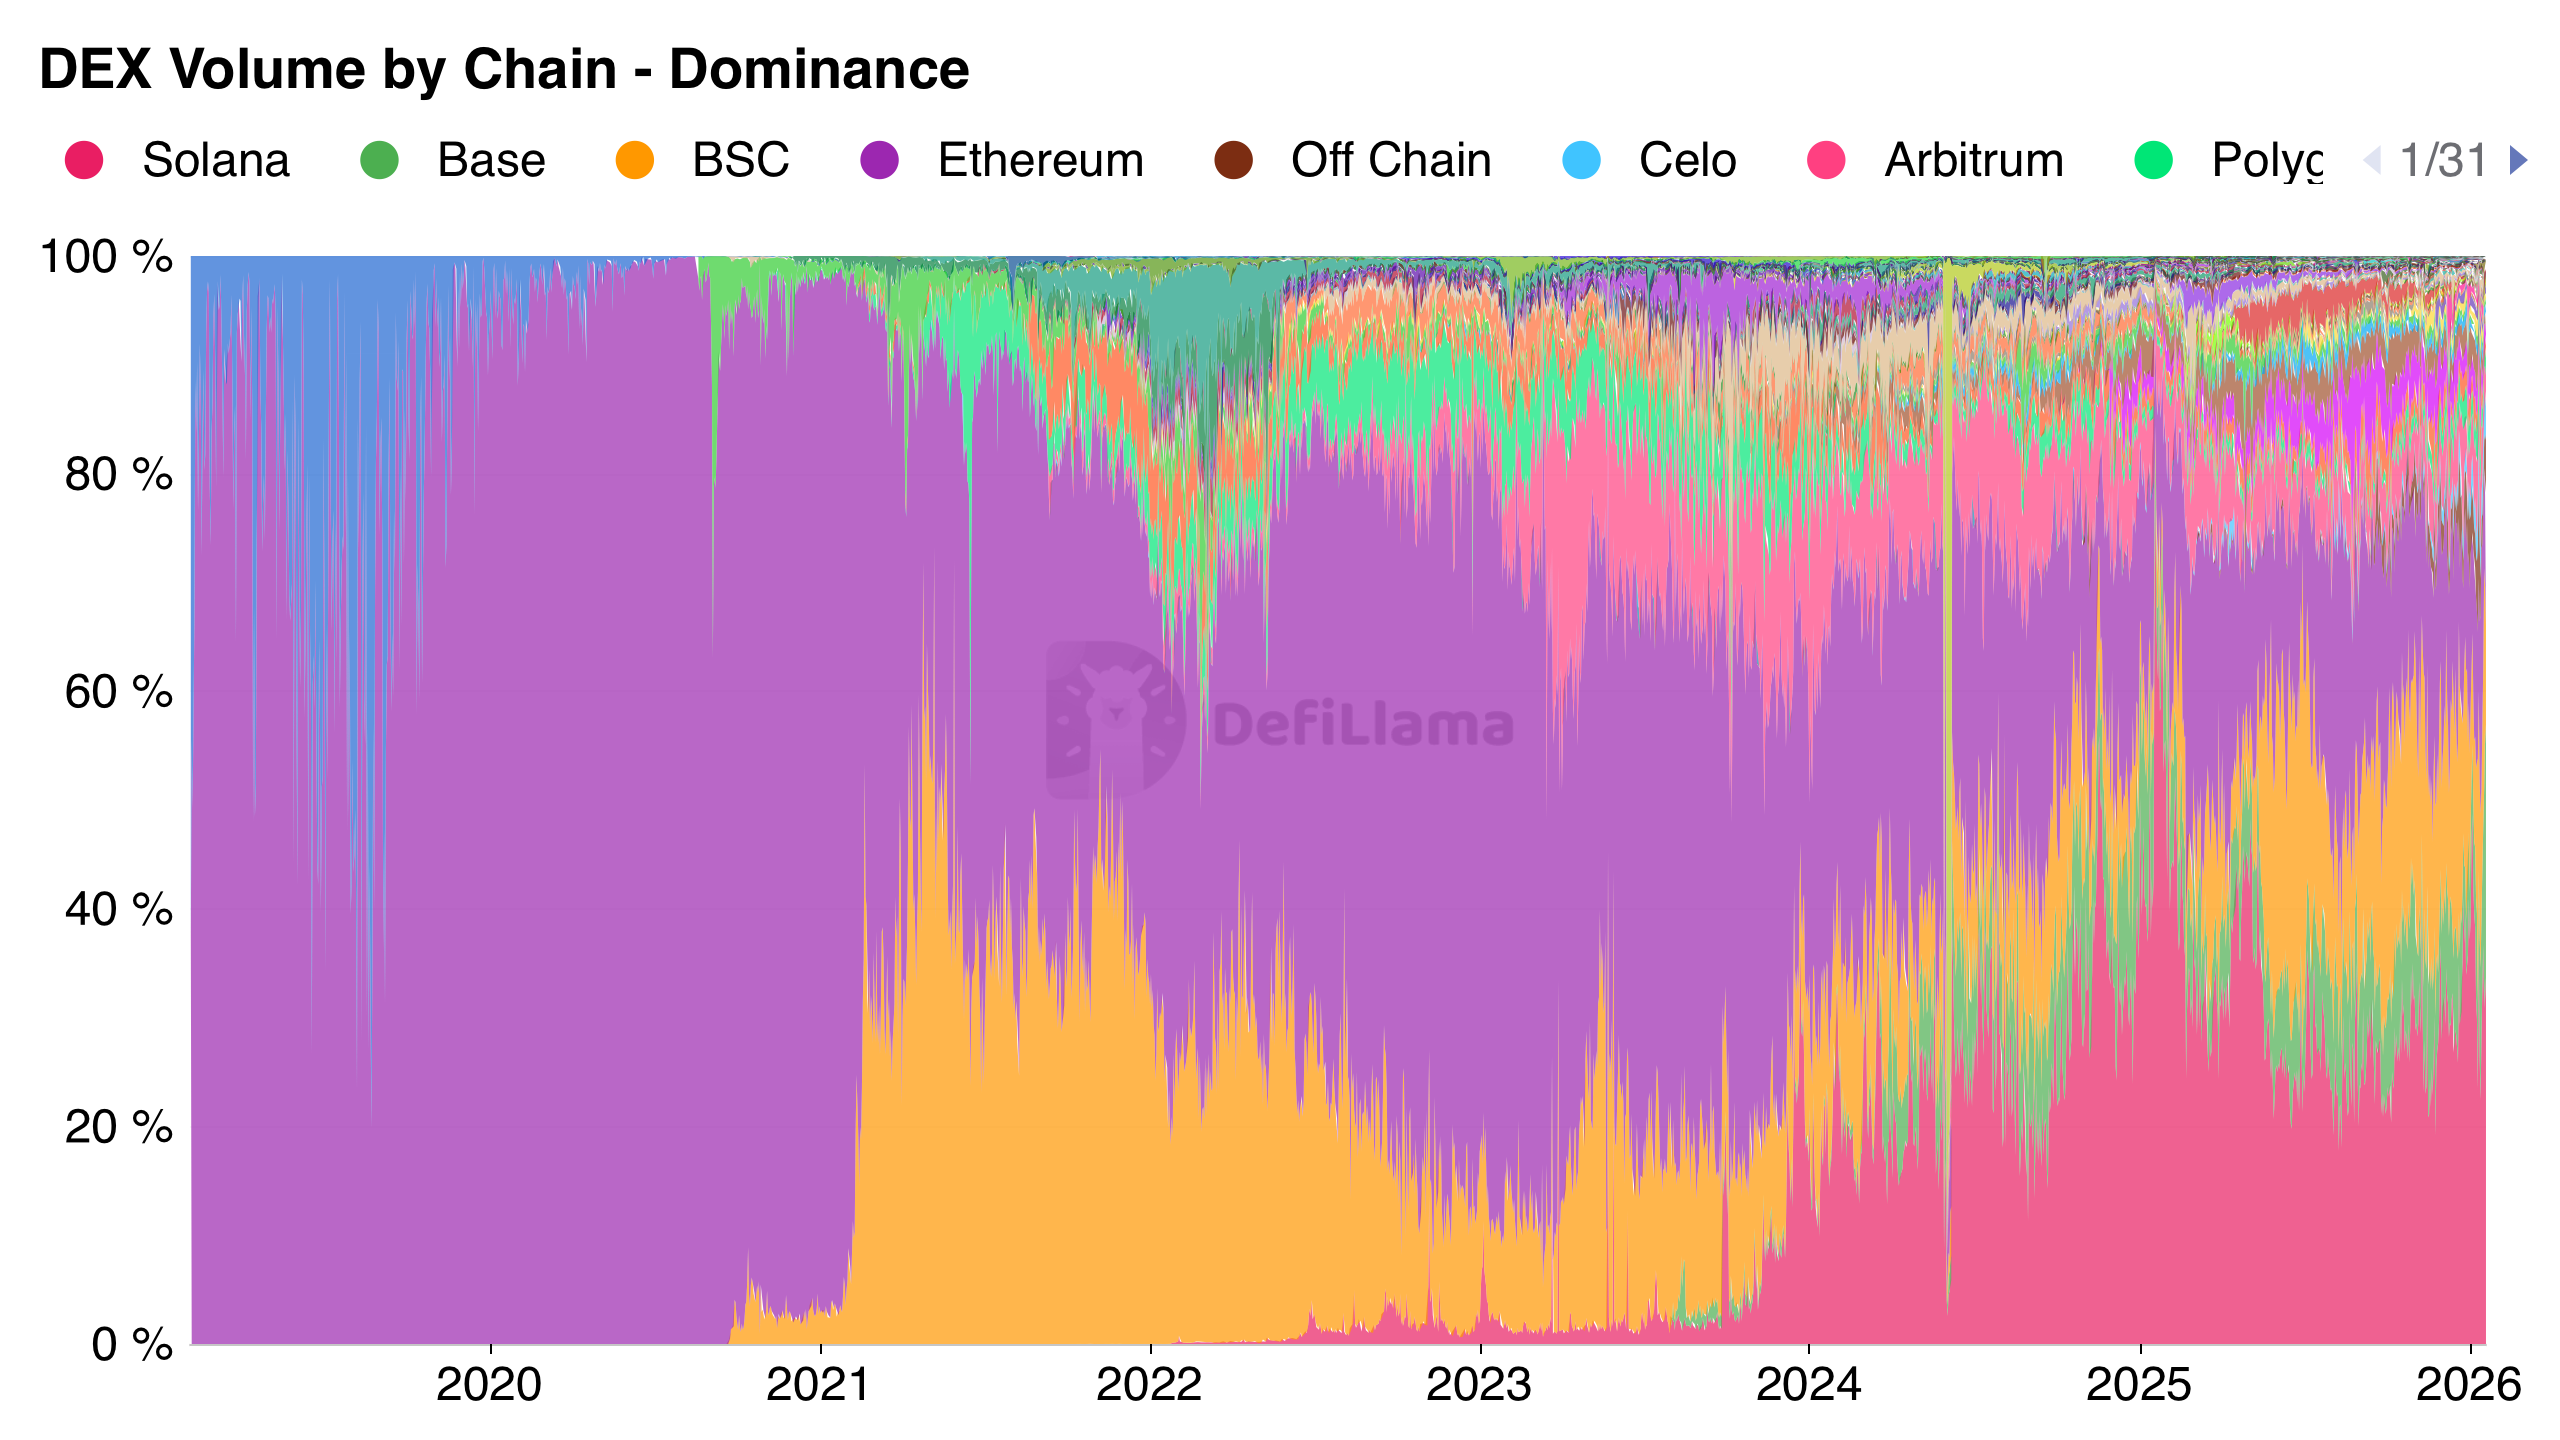
\includegraphics[width=1\textwidth]{Figures/DEX Volume ByChain.png}
  \end{figure}
  \textbf{Perspective}: Solana holds the relative majority of DEX volume; Ethereum is second (as of January 2026).
\end{frame}

%----------------------------------------------------------------------------------------
\section{Lending Protocols}
%----------------------------------------------------------------------------------------

\begin{frame}{DeFi Lending: The Basics}
  Traditional lending requires credit checks because loans are \textit{under}-collateralised---you borrow more than you put down.
  
  \vspace{1em}
  DeFi lending is \highlight{over-collateralised}: You must deposit more value than you borrow.
  
  \vspace{1em}
  \textbf{Example} (Aave):
  \begin{itemize}
    \item Deposit 10 ETH as collateral (worth \$30,000)
    \item Borrow up to $\approx$75\% in stablecoins: \$22,500 USDC
    \item Pay interest on the borrowed amount
    \item Earn interest on your deposited collateral
  \end{itemize}
  
  \vspace{1em}
  \textbf{Why would anyone do this?}
  \begin{itemize}
    \item Get liquidity without selling (tax event, bullish on ETH)
    \item Leverage: Use borrowed funds to buy more ETH
    \item Yield farming: Deploy borrowed funds in other protocols
  \end{itemize}
\end{frame}

\begin{frame}{How Lending Protocols Work}
  \textbf{Key participants}:
  \begin{itemize}
    \item \textbf{Lenders}: Deposit assets into pools, earn interest
    \item \textbf{Borrowers}: Deposit collateral, borrow from pools, pay interest
    \item \textbf{Liquidators}: Monitor undercollateralised positions, liquidate for profit
  \end{itemize}
  
  \vspace{1em}
  \textbf{Interest rates} are set algorithmically based on \highlight{utilisation}:
  \[
  \text{Utilisation} = \frac{\text{Total Borrowed}}{\text{Total Deposited}}
  \]
  
  \begin{itemize}
    \item Low utilisation (lots of idle capital): Low rates to encourage borrowing
    \item High utilisation (capital scarce): High rates to attract deposits
  \end{itemize}
  
  \vspace{0.5em}
  This is supply and demand encoded in a smart contract.
\end{frame}

\begin{frame}{The Health Factor and Liquidations}
  \textbf{Health Factor}: A measure of how safe your position is.
  \[
  \text{Health Factor} = \frac{\text{Collateral Value} \times \text{Liquidation Threshold}}{\text{Borrowed Value}}
  \]
  
  \vspace{0.5em}
  \textbf{Example}: 
  \begin{itemize}
    \item Collateral: 10 ETH @ \$3,000 = \$30,000
    \item Liquidation threshold: 80\%
    \item Borrowed: \$20,000 USDC
    \item Health Factor: $(30{,}000 \times 0.80) / 20{,}000 = \highlight{1.2}$
  \end{itemize}
  
  \vspace{0.5em}
  \textbf{If ETH drops to \$2,500}:
  \begin{itemize}
    \item Collateral: \$25,000
    \item Health Factor: $(25{,}000 \times 0.80) / 20{,}000 = \bad{1.0}$
  \end{itemize}
  
  \vspace{0.5em}
  \textbf{At Health Factor $<$ 1}: the position becomes \highlight{liquidatable}. Liquidators repay part of the debt and seize collateral at a discount ($\approx$5--10\%).
\end{frame}

\begin{frame}{Liquidation Cascades}
  \textbf{The danger}: Liquidations can trigger more liquidations.
  
  \vspace{1em}
  \textbf{Scenario}:
  \begin{enumerate}
    \item ETH price drops sharply
    \item Many positions become undercollateralised
    \item Liquidators seize and sell ETH collateral
    \item This selling pressure pushes ETH price lower
    \item More positions become undercollateralised
    \item Repeat...
  \end{enumerate}
  
  \vspace{1em}
  This is a \highlight{liquidation cascade}---a feedback loop that amplifies price drops.
  
  \vspace{0.5em}
  
  \textbf{Real example}: On May 19, 2021, over \$800 million was liquidated across DeFi in 24 hours during a market crash.
\end{frame}

\begin{frame}{Major Lending Protocols}
  \begin{center}
  \begin{tabular}{lcc}
    \toprule
    \textbf{Protocol} & \textbf{TVL (2024)} & \textbf{Key Feature} \\
    \midrule
    Aave & $\approx$\$10B & Multi-chain, flash loans \\
    Compound & $\approx$\$2B & Pioneer, simple design \\
    MakerDAO & $\approx$\$8B & Issues DAI stablecoin \\
    \bottomrule
  \end{tabular}
  \end{center}
  
  \vspace{1em}
  \textbf{MakerDAO} is special: Instead of borrowing existing tokens, you mint new DAI stablecoins against your collateral. This creates currency rather than lending it.
  
  \vspace{0.5em}
  We'll explore stablecoins in depth in Topic 5.
  
  \vspace{1em}
  \textbf{Note}: Despite being ``decentralised,'' these protocols have governance tokens and upgrade mechanisms that introduce some centralisation.
\end{frame}

%----------------------------------------------------------------------------------------
\section{Oracles: The Data Problem}
%----------------------------------------------------------------------------------------

\begin{frame}{Why DeFi Needs Oracles}
  Recall from Topic 3: Smart contracts can only access data on the blockchain.
  
  \vspace{1em}
  \textbf{But DeFi needs external data}:
  \begin{itemize}
    \item \textbf{Lending}: What's the current price of ETH? (For liquidations)
    \item \textbf{Derivatives}: What's the S\&P 500 level? (For settlement)
    \item \textbf{Insurance}: Did the flight get cancelled? (For payouts)
  \end{itemize}
  
  \vspace{1em}
  \begin{block}{Oracle}
    A service that feeds external data to smart contracts.
  \end{block}
  
  \vspace{0.5em}
  \textbf{The trust problem}: The entire DeFi system can be ``trustless,'' but if the oracle lies about prices, contracts execute on false data.
  
  \vspace{0.5em}
  Oracles are a critical piece of infrastructure---and a major attack vector.
\end{frame}

\begin{frame}{How Chainlink Works}
  \textbf{Chainlink} is the dominant oracle provider in DeFi.
  
  \vspace{1em}
  \textbf{Basic architecture}:
  \begin{enumerate}
    \item Multiple independent node operators fetch data from off-chain sources
    \item Each node signs and submits their answer on-chain
    \item The protocol aggregates answers (typically median)
    \item Smart contracts read the aggregated price
  \end{enumerate}
  
  \vspace{1em}
  \textbf{Security model}:
  \begin{itemize}
    \item No single node can manipulate the price
    \item Nodes are incentivised with LINK tokens
    \item Nodes stake LINK that can be slashed for bad behaviour
    \item Reputation systems track node reliability
  \end{itemize}
  
  \vspace{0.5em}
  This is ``decentralised'' trust---you trust the network of oracles rather than any single data provider.
\end{frame}

\begin{frame}{Oracle Attacks}
  \textbf{If you can manipulate the oracle, you can drain the protocol.}
  
  \vspace{1em}
  \textbf{Attack types}:
  
  \vspace{0.5em}
  \textbf{1. Spot price manipulation}:
  \begin{itemize}
    \item If a protocol uses a single DEX as its price source...
    \item Attacker manipulates that DEX price temporarily
    \item Borrows/liquidates at the manipulated price
    \item Returns the market to normal
  \end{itemize}
  
  \vspace{0.5em}
  \textbf{2. Flash loan attacks} (more on this later):
  \begin{itemize}
    \item Borrow millions with no collateral
    \item Use funds to manipulate prices
    \item Exploit protocol at bad prices
    \item Repay loan, pocket profit---all in one transaction
  \end{itemize}
  
  \vspace{0.5em}
  \textbf{Mitigation}: Use time-weighted average prices (TWAP), multiple oracle sources, and circuit breakers.
\end{frame}

\begin{frame}{The Oracle Landscape}
  \begin{center}
  \begin{tabular}{lp{6.5cm}}
    \toprule
    \textbf{Provider} & \textbf{Approach} \\
    \midrule
    Chainlink & Decentralised node network, most widely used \\
    Uniswap TWAP & Time-weighted average from on-chain trades \\
    Pyth & High-frequency data from trading firms \\
    Band Protocol & Chainlink competitor, different chain focus \\
    \bottomrule
  \end{tabular}
  \end{center}
  
  \vspace{1em}
  \textbf{Open questions}:
  \begin{itemize}
    \item How decentralised are ``decentralised'' oracles really?
    \item Who bears liability if oracle data is wrong?
    \item Can oracles scale to support high-frequency DeFi?
  \end{itemize}
  
  \vspace{0.5em}
  Oracles remain one of the most critical---and most debated---pieces of DeFi infrastructure.
\end{frame}

%----------------------------------------------------------------------------------------
\section{DeFi Risks and Failures}
%----------------------------------------------------------------------------------------

\begin{frame}{Categories of DeFi Risk}
  \begin{center}
  \begin{tabular}{lp{6cm}}
    \toprule
    \textbf{Risk Type} & \textbf{Examples} \\
    \midrule
    Smart contract & Bugs, exploits, reentrancy attacks \\
    Economic design & Flawed incentives, death spirals \\
    Oracle & Price manipulation, stale data \\
    Governance & Malicious proposals, vote buying \\
    Liquidity & Bank runs, liquidation cascades \\
    Composability & Failures propagate across protocols \\
    Regulatory & Legal uncertainty, enforcement actions \\
    \bottomrule
  \end{tabular}
  \end{center}
  
  \vspace{1em}
  \textbf{Scale of losses}: Over \$3 billion was lost to DeFi exploits in 2022 alone.
  
  \vspace{0.5em}
  Unlike traditional finance, there's usually no insurance, no bailout, and no recourse.
\end{frame}

\begin{frame}{Flash Loans: A Double-Edged Sword}
  \begin{block}{Flash Loan}
    A loan that must be borrowed and repaid within the same transaction. No collateral required.
  \end{block}
  
  \vspace{0.5em}
  \textbf{How it works}:
  \begin{enumerate}
    \item Borrow \$100 million from Aave (no collateral)
    \item Do something with the funds (arbitrage, liquidation, etc.)
    \item Repay \$100 million + small fee
    \item If you can't repay, entire transaction reverts as if nothing happened
  \end{enumerate}
  
  \vspace{0.5em}
  \textbf{Legitimate uses}: Arbitrage, collateral swaps, self-liquidation
  
  \vspace{0.5em}
  \textbf{Attack vector}: Anyone can temporarily access massive capital to:
  \begin{itemize}
    \item Manipulate prices on low-liquidity markets
    \item Exploit economic design flaws
    \item Attack governance votes
  \end{itemize}
  
  Many major DeFi exploits have used flash loans as the funding mechanism.
\end{frame}


\begin{frame}{Case Study: Terra/Luna Collapse (May 2022)}
\begin{figure}
    \centering
   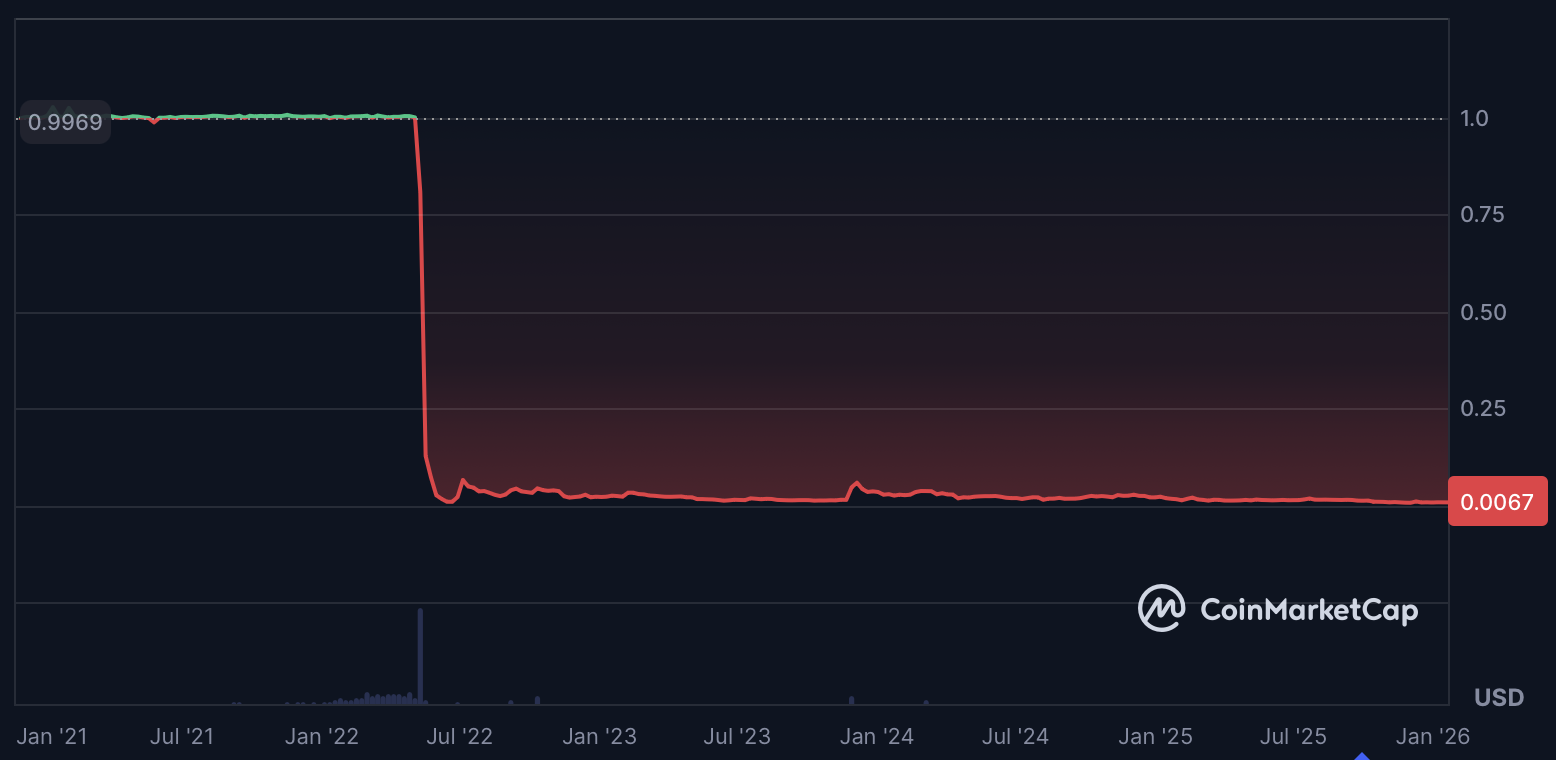
\includegraphics[width=1\textwidth]{Figures/UST price.png}
\end{figure}
  \textbf{Figure}: Exchange rate between UST and USD (as of January 2026). 
\end{frame}

\begin{frame}{Case Study: Terra/Luna Collapse (May 2022)}
  \textbf{Background}: Terra was a blockchain with an algorithmic stablecoin (UST) designed to maintain a \$1 peg through arbitrage with LUNA tokens.
  
  \vspace{0.5em}
  \textbf{The mechanism}:
  \begin{itemize}
    \item UST $>$ \$1: Mint UST by burning LUNA (increases UST supply)
    \item UST $<$ \$1: Burn UST to mint LUNA (decreases UST supply)
    \item Anchor protocol paid 20\% APY on UST deposits
  \end{itemize}
  
  \vspace{0.5em}
  \textbf{The collapse}:
  \begin{enumerate}
    \item Large UST withdrawals broke the peg slightly
    \item Panic led to more UST selling
    \item UST $\rightarrow$ LUNA arbitrage massively inflated LUNA supply
    \item LUNA price collapsed (from \$80 to \$0.0001)
    \item Without valuable LUNA, UST had no backing
    \item Death spiral: $\approx$\$60 billion in value destroyed in days
  \end{enumerate}
\end{frame}

\begin{frame}{Lessons from Terra/Luna}
  \textbf{What went wrong}:
  \begin{itemize}
    \item Circular backing: UST was backed by LUNA, whose value depended on UST demand
    \item Unsustainable yields: 20\% APY attracted capital but was paid from reserves
    \item No external collateral: Nothing outside the system to absorb shocks
    \item Reflexive death spiral: The mechanism that was supposed to restore the peg instead accelerated collapse
  \end{itemize}
  
  \vspace{1em}
  \textbf{Broader lessons}:
  \begin{itemize}
    \item ``Algorithmic'' doesn't mean safe---it means the risks are encoded in code
    \item High yields often signal high risk (or unsustainable subsidies)
    \item Circular dependencies create fragility
    \item Stablecoins need robust collateral (Topic 5)
  \end{itemize}
  
  \vspace{0.5em}
  Terra's collapse accelerated regulatory scrutiny of stablecoins worldwide.
\end{frame}

\begin{frame}{The ``Decentralisation Illusion''}
  DeFi markets itself as decentralised, but centralisation persists:
  
  \vspace{1em}
  \textbf{Points of centralisation}:
  \begin{itemize}
    \item \textbf{Development teams}: Small groups control upgrades
    \item \textbf{Governance tokens}: Often concentrated among VCs and founders
    \item \textbf{Oracles}: Most protocols depend on Chainlink
    \item \textbf{Stablecoins}: USDC can freeze addresses (and has)
    \item \textbf{Frontends}: Most users access DeFi through centralised websites
    \item \textbf{Infrastructure}: Infura, Alchemy handle most node traffic
  \end{itemize}
  
  \vspace{1em}
  \textbf{Implication}: DeFi has reduced some intermediaries but created new dependencies. ``Trustless'' is often aspirational rather than actual.
  
  \vspace{0.5em}
  This doesn't make DeFi useless---but claims should be evaluated critically.
\end{frame}

\begin{frame}{Systemic Risk: DeFi and Traditional Finance}
  \textbf{Currently}: DeFi is largely isolated from traditional banking.
  \begin{itemize}
    \item Banks have minimal direct crypto exposure
    \item Most DeFi users are crypto-native
  \end{itemize}
  
  \vspace{1em}
  \textbf{Growing connections}:
  \begin{itemize}
    \item Bitcoin and Ethereum ETFs (approved 2024)
    \item Banks offering crypto custody
    \item Stablecoins backed by bank deposits and treasuries
    \item Institutional DeFi participation increasing
  \end{itemize}
  
  \vspace{1em}
  \textbf{Potential spillover channels}:
  \begin{itemize}
    \item Stablecoin runs could stress money markets
    \item Crypto crashes could hit institutional portfolios
    \item Leverage in DeFi could amplify traditional market moves
  \end{itemize}
  
  \vspace{0.5em}
  Regulators are increasingly focused on these connections.
\end{frame}

%----------------------------------------------------------------------------------------
\section{Summary and Next Steps}
%----------------------------------------------------------------------------------------

\begin{frame}{Key Takeaways}
  \begin{enumerate}
    \item \textbf{DeFi replaces intermediaries with smart contracts}
    \begin{itemize}
      \item Permissionless, transparent, composable---but also risky
    \end{itemize}
    
    \vspace{0.3em}
    \item \textbf{AMMs enable trading without order books}
    \begin{itemize}
      \item Constant product formula: $x \cdot y = k$
      \item LPs earn fees but face impermanent loss
    \end{itemize}
    
    \vspace{0.3em}
    \item \textbf{Lending is over-collateralised with algorithmic rates}
    \begin{itemize}
      \item Liquidations enforce solvency but can cascade
    \end{itemize}
    
    \vspace{0.3em}
    \item \textbf{Oracles are critical infrastructure---and attack vectors}
    \begin{itemize}
      \item Chainlink dominant; price manipulation is real
    \end{itemize}
    
    \vspace{0.3em}
    \item \textbf{DeFi carries substantial risks}
    \begin{itemize}
      \item Smart contract bugs, economic design flaws, Terra collapse
      \item ``Decentralisation'' is often partial
    \end{itemize}
  \end{enumerate}
\end{frame}

\begin{frame}{What's Next}
  \textbf{Topic 5: Stablecoins and Central Bank Digital Currencies}
  \begin{itemize}
    \item Types of stablecoins (fiat-backed, crypto-backed, algorithmic)
    \item How USDC, USDT, DAI work
    \item Stablecoin risks and regulation
    \item Central Bank Digital Currencies (CBDCs)
    \item The future of money
  \end{itemize}
  
  \vspace{1em}
  \textbf{Preparation}:
  \begin{itemize}
    \item Think about: What makes ``stable'' coins stable---and what can break that stability?
    \item Explore: Look at stablecoin market caps on CoinGecko---which are largest?
  \end{itemize}
\end{frame}

\begin{frame}[plain]
  \vfill
  \begin{center}
    {\Large Questions?}
  \end{center}
  \vfill
\end{frame}

\end{document}